\section{Photon Mulitplicity Detector (PMD)}

	Ο Photon Multiplicity Detector (PMD) του STAR, καλύπτει περιοχές pseudorapidity $2.3<\eta<2.5$, $\Delta \phi=2\pi$ και $p_t$ μικρή εως και 25MeV/c και θα μετράει την χωρική κατανομή των φωτονίων προκείμένου να μελετησει την ροή και τις διακυμάνσεις της.
	Χρησιμοποιείται έναντι των καλοριμέτρων σε περιοχές υψηλής πυκνότητας καθώς αν η περιοχή είναι πυκνή σε τροχιές, τότε οι καταιγισμοί των δευτερεύοντων σωματιδίων θα αλληλοεπικαλύπτονταν και ένα καλορίμετρο δεν θα μπορούσε να τις ξεχωρίσει. 
	Ας δούμε ποιοτικά την λειτουργία του PDM. 
	
	Η βασική δομή του PMD φαίνεται στην Εικόνα (\ref{fig3.24}).   
     Απαρτίζεται από διακριτά στοιχεία που είναι τοποθετημένα πίσω από ένα στρώμα μολύβδου. Τα φωτόνια που περνούν μέσα από το στρώμα του μολύβδου ξεκινούν έναν ηλεκτρομαγνητικό καταιγισμό και παράγουν ισχυρά σήματα. Αυτά τα σήματα δημιουργούνται στις κυψελίδες που υπάρχουν στα ευαίσθητα σημεία του ανιχνευτή. Η διαφορά με τα φορτισμένα αδρόνια είναι ότι εκείνα επηρεάζουν συνθήθως μόνο μία κυψελίδα, διότι δεν προκλούν καταιγισμό και έτσι παράγουν σήμα που αντιστοιχεί σε MIP. 
	To πάχος του μολυβδου είναι επιλεγμένο έτσι ώστε να παρέχει την βέλτιστη ισορροπία μεταξύ υψηλής πιθανότητας τα φωτόνια να κάνουν καταιγισμό και επίτευξη όσο το δυνατόν στενότερου πάχους για κάθε καταιγισμό ώστε να μειωθούν έχουμε αλληλοεπικαλύψεις καθώς θα υπάρχει περιβάλλον υψηλής πυκνότητας.
	Ακόμη, πριν από το κύριο τμήμα του ανιχνευτή, υπάρχει και ένα άλλο στρώμα, ο Veto Detector. Αυτός συνεισφέρει στο να εμποδίζει τα φορτισμένα σωματίδια απ΄ το να εισέρχονται στην περιχοή του μολύβδου όπου ξεκινάνε οι καταιγισμοί.
	\begin{figure}[h!]
		\centering
		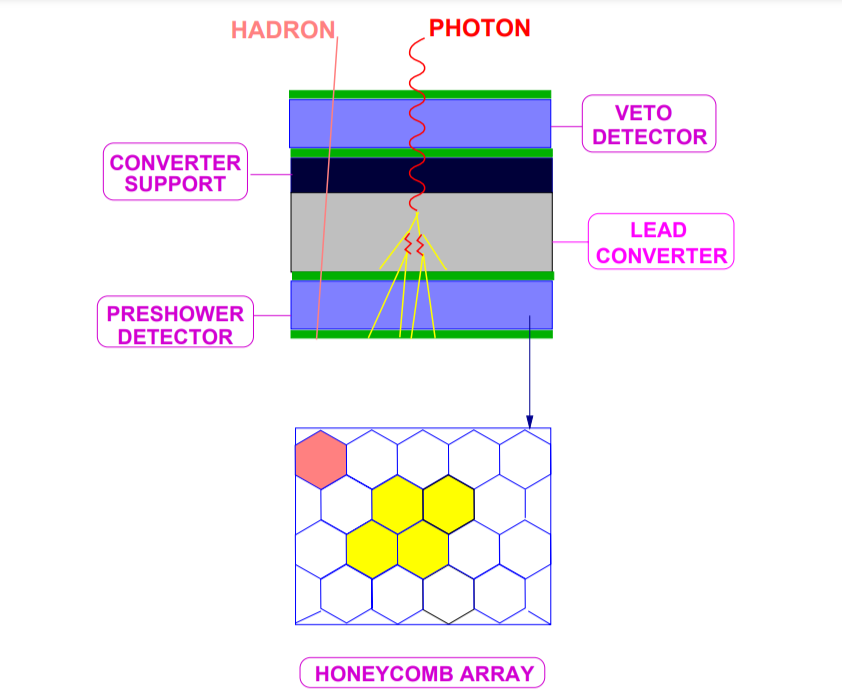
\includegraphics[scale=0.4]{STAR_Detectors/PMD_principle}
		\caption{Η βασική δομή και λειτουργία του PMD}
		\label{fig3.24}
	\end{figure}
	
	Τόσο ο Veto όσο και το ευαίσθητο τμήμα του PMD (Preshower Detector) αποτελούνται από εξαγωνικές κυψελίδες τοποθετημένες σε διάταξη κηρύθρας και η καθεμία είναι θάλαμος αερίων που λειτουργεί σε αναλογική περιοχή (ενδεικτικά στον Preshower υπάρχει μείγμα Ar/$CO_2$). 
	Ο σκελετός που αποτελεί τα όρια των κυψελίδων στην κηρύθρα είναι φτιαγμένος από χαλκό και ταυτόχρονα λειτουργεί ως κάθοδος αφού τον τοποθετούμε σε χαμηλό δυναμικό σε σχέση με το σύρμα ανόδου που υπάρχει στο κέντρο της κάθε κυψελίδας. 
	Μία συστοιχία από 24x24 κυψελίδες αποτελεί ένα \textit{module} και έχει ρομβικό σχήμα με πλευρά 254mm. Επίσης, κάποια modules από 4-9 είναι κλεισμένα εντός ενός αεροστεγούς θαλάμου ο οποίος αποτελεί το \textit{supermodule}. Συνολικά ο PMD αποτελείται από 24 supermodules. Στην Εικόνα (\ref{fig3.25}) φαίνεται η δομή μίας κυψελίδας καθώς και η συνολική εξαγωνική διάταξη των supermodules.
	
	\begin{figure}[h!]
		\centering
		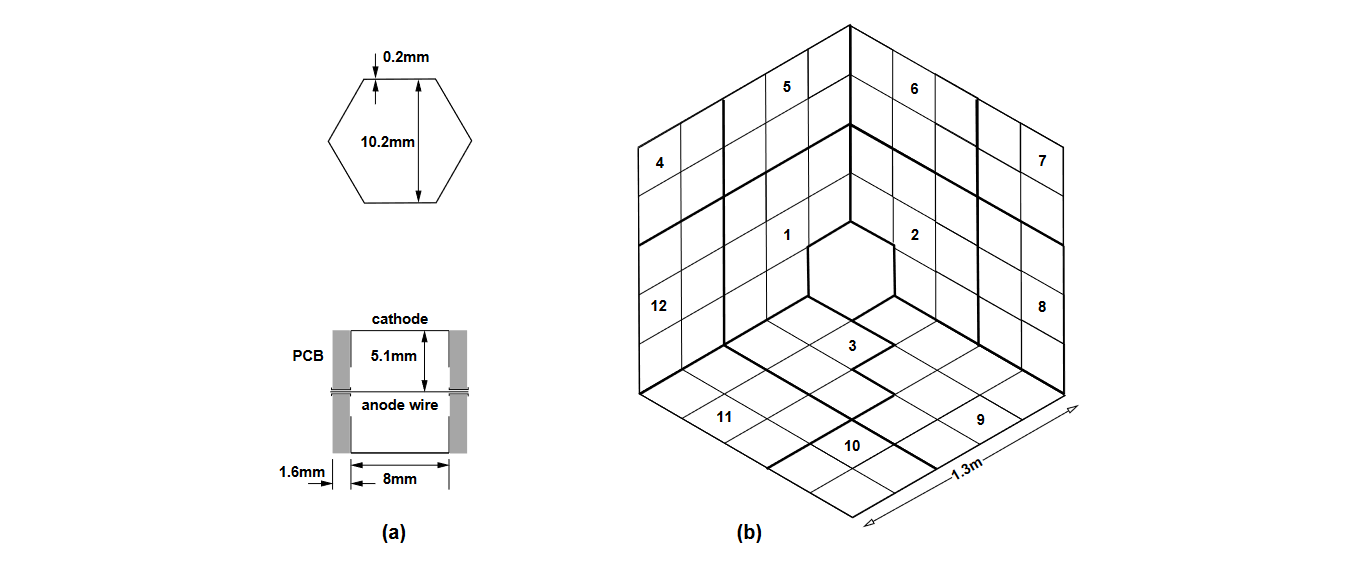
\includegraphics[scale=0.5]{STAR_Detectors/PMD_layout}
		\caption{(a) Δομή μίας κυψελίδας, (b) Διάταξη των modules σε supermodules η οποία καταλήγει σε ένα εξαγωνικό σχήμα.}
		\label{fig3.25}
	\end{figure}
	
	Όλες οι επιλογές των μερών που απαρτίζουν τον PMD έγιναν με γνώμονα τρεις στόχους, προκειμένου να είναι διαχειρήσιμη η υψηλή πυκνότητα εισερχόμενων σωματιδίων. Το σήμα των MIPs πρέπει να είναι περιορισμένο σε μία κυψελίδα, τα δ-ηλεκτρόνια με χαμηλή ενέργεια πρέπει να εμποδιστούν απ' το να ταξιδεύουν εως τις γειτονικές κυψελίδες προκαλώντας ανεπιθύμητη μεταφορά σήματος μεταξύ τους και τέλος η πιθανότητα ένα σωματίδιο να δώσει σήμα σε πολλές κυψελίδες να γίνει ελάχιστη.